\begin{figure} [H]
	\begin{center}
		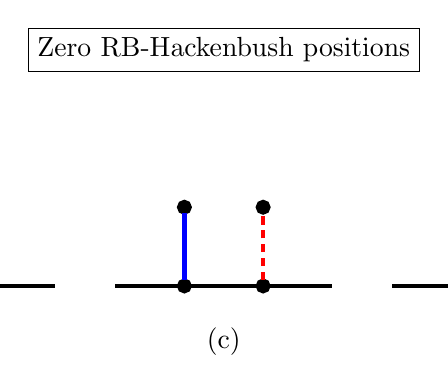
\begin{tikzpicture}
			\node[draw] (title) at (1.5, 3) {Zero RB-Hackenbush positions};
			\node (p1) at (0,0) {};
			\node (p2) at (3,0) {};
			\begin{scope} [ultra thick, every node/.style={scale=0.4, circle, draw, fill=black}]
				\node (p3) at (1,0) {};
				\node (p4) at (1,1) {};
				\node (p6) at (2,0) {};
				\node (p7) at (2,1) {};
				\draw (p1) -- (p2);
				\draw[blue] (p3) -- (p4);
				\draw[red, densely dashed] (p6) -- (p7);
			\end{scope}
			\coordinate[thick, label=(c)] () at (1.5, -1);
			\hspace{-200pt}{ \begin{scope} [ultra thick, every node/.style={scale=0.4, circle, draw, fill=black}]
				\draw (p1) -- (p2);
			\end{scope}}
			\coordinate[thick, label=(a)] () at (1.5, -1);
			\hspace{100pt}{ \begin{scope} [ultra thick, every node/.style={scale=0.4, circle, draw, fill=black}]
				\node (p3) at (1,0) {};
				\node (p4) at (1,1) {};
				\node (p5) at (1,2) {};
				\node (p6) at (1.5,0) {};
				\node (p7) at (1.5,1) {};
				\node (p8) at (2, 0) {};
				\node (p9) at (2, 1) {};
				\draw (p1) -- (p2);
				\draw[blue] (p3) -- (p4);
				\draw[blue] (p4) -- (p5);
				\draw[red, densely dashed] (p6) -- (p7);
				\draw[red, densely dashed] (p8) -- (p9);
			\end{scope}}
			\coordinate[thick, label=(b)] () at (1.5, -1);
			\hspace{200pt}{ \begin{scope} [ultra thick, every node/.style={scale=0.4, circle, draw, fill=black}]
				\node (p3) at (1,0) {};
				\node (p4) at (1,1) {};
				\node (p5) at (1,2) {};
				\node (p6) at (2,0) {};
				\node (p7) at (2,1) {};
				\node (p8) at (2,2) {};
				\draw (p1) -- (p2);
				\draw[blue] (p3) -- (p4);
				\draw[red, densely dashed] (p4) -- (p5);
				\draw[red, densely dashed] (p6) -- (p7);
				\draw[blue] (p7) -- (p8);
			\end{scope}}
			\coordinate[thick, label=(d)] () at (1.5, -1);
			\hspace{100pt}{ \begin{scope} [ultra thick, every node/.style={scale=0.4, circle, draw, fill=black}]
				\node (p3) at (1,0) {};
				\node (p4) at (1,1) {};
				\node (p6) at (2,0) {};
				\node (p7) at (2,1) {};
				\node (p8) at (1.5,2) {};
				\draw (p1) -- (p2);
				\draw[blue] (p3) -- (p4);
				\draw[red, densely dashed] (p4) -- (p8);
				\draw[red, densely dashed] (p6) -- (p7);
				\draw[blue] (p7) -- (p8);
			\end{scope}}
			\coordinate[thick, label=(e)] () at (1.5, -1);
		\end{tikzpicture}
	\end{center}
	\caption{}
\end{figure}